\providecommand{\thebibpath}{..}
\makeatletter\def\input@path{{\thebibpath/}{.}}\makeatother
\documentclass[main.tex]{subfiles}
\begin{document}

\section{Mechanical}

	The robot frame is made out of CNC-cut copper-coated fibreglass, known more commonly for its use in prototyping circuitry.
	This has the advantage of being light yet stiff, and immune to plastic deformation.

	Two MAXON motors \cite{motor} are attached to the robot, each with a corresponding 14:1 gearbox \cite{gearbox} and 512 count-per-revolution encoder \cite{encoder}.
	The first motor is connected via a timing belt with a 40:16 ratio to the drive wheel, while the second motor is directly attached to a steel flywheel (henceforth referred to as the \enquote{turntable}).

	To prevent damage to the turntable motor shaft, the chassis of the robot shields the turntable from direct impact, reinforced with some metal bolts.
	Atop this shielding, lies the control board on the front side of the robot, and the battery duct-taped to the rear.

	Previous work concluded \cite[p.~54]{aleksi} that a better simulation model of the unicycle was desirable, to help determine whether poor learning progress was due to implementation errors in software, or simply due to the small unicycle having a more challenging set of dynamics than the previously-simulated large unicycle.

	As part of my project, model parameters were found for the small unicycle, shown alongside the method used to obtain them in \cref{table:mechanical}.
	Noting that since one of the goals of \textsc{Pilco} is \emph{not} to require a detailed system model, some properties were simply estimated.

	\begin{table}
		{
\small
\renewcommand{\arraystretch}{1.5}
\begin{tabularx}{\linewidth}{
	@{}
	r
	>{\raggedright}p{0.25\linewidth}
	S[
		scientific-notation = engineering,
		table-format=-3e-1,
		table-auto-round
	]
	s
	X
	@{}
}
\toprule
 & Description & \multicolumn{2}{c}{Value} & Determined by \\
\midrule
	\texttt{mt}
		& Mass of turntable (tt.)
		& 0.2110 & \kilogram
		& estimation using $\rho_\mathrm{steel} = 8000\si{\kilogram\per\cubic\meter}$.
	\\
	\texttt{mw}
		& Mass of wheel and axle
		& 0.1090 & \kilogram
		& direct measurement, by detaching the axle bearings, and suspending the robot frame such that it does not exert any reaction force on the axle.
	\\
	\texttt{mf}
		& Mass of frame
		& 0.6600 & \kilogram
		& subtracting from the total mass of \SI{0.98}{\kilogram}.
	\\
\midrule
	\texttt{rw}
		& Radius of wheel
		& 0.0353 & \meter
		& measuring the wheel circumference as \SI{22.2}{\centi\meter}.
	\\
	\texttt{rf}
		& Distance from COM of frame to wheel
		& 0.0800 & \meter
		&\tikzmark{bra1}\multirow{3}{\hsize}{%
			finding the balancing point of the robot, by suspending from a string.
		}
	\\
	\texttt{rt}
		& Distance from COM of frame to turntable
		& 0.0070 & \meter
		& \tikzmark{brb1}
	\\
\midrule
	\texttt{Cw}
		& MOI of wheel $\parallel$ to axle
		& 3.0536e-07 & \kilogram \square\meter
		&\tikzmark{bra2}\multirow{2}{\hsize}{%
			computing $m_\mathrm{wheel} = \mathtt{mw} - \rho_\mathrm{steel} \pi \allowbreak(lr^2)_\textrm{axle}$, and then assuming a uniform laminar disc.
		}
	\\
	\texttt{Aw}
		& MOI of wheel $\bot$ to axle
		& 1.2739e-04 & \kilogram \square\meter
		& \tikzmark{brb2}
	\\
	\texttt{Cf}
		& MOI of frame
		& 5.1116e-04 & \kilogram \square\meter
		&\tikzmark{bra3}\multirow{3}{\hsize}{%
			estimation by dimensional analysis, assuming that $I \propto \mathtt{mf}\,\mathtt{rf}^2$, and using known values for the large unicycle.
		}
	\\
	\texttt{Bf}
		& MOI of frame
		& 2.8406e-04 & \kilogram \square\meter
		&
	\\
	\texttt{Af}
		& MOI of frame
		& 2.618e-04 & \kilogram \square\meter
		& \tikzmark{brb3}
	\\
	\texttt{Ct}
		& MOI of tt. $\parallel$ to axle
		& 1.611e-04 & \kilogram \square\meter
		&\tikzmark{bra4}\multirow{2}{\hsize}{%
			decomposition into cylinders, and using $\rho_\mathrm{steel}$.
		}
	\\
	\texttt{At}
		& MOI of tt. $\bot$ to axle
		& 8.102e-05 & \kilogram \square\meter
		& \tikzmark{brb4}
	\\
\midrule
	\texttt{maxU}
		& Maximum input torques
		& {
			\renewcommand{\arraystretch}{1}
			$\begin{bmatrix}0.205 \\ 0.513\end{bmatrix}$
		} & \newton \meter
		& applying the gearing ratios~\cite{gearbox} to the torque limits quoted on the datasheet~\cite{motor}.
	\\
\bottomrule
\end{tabularx}
\begin{tikzpicture}[overlay, remember picture]
	\draw [decoration={brace,amplitude=0.5em},decorate,thick,black]
		let \p1=(bra1.mid), \p2=(brb1.mid) in
			({\x1 - 0.8em}, {\y1 +0.5em}) -- node[right=0.6em] {} ({\x1 - 0.8em}, {\y2 - 0.5em});
	\draw [decoration={brace,amplitude=0.5em},decorate,thick,black]
		let \p1=(bra2.mid), \p2=(brb2.mid) in
			({\x1 - 0.8em}, {\y1 +0.5em}) -- node[right=0.6em] {} ({\x1 - 0.8em}, {\y2 - 0.5em});
	\draw [decoration={brace,amplitude=0.5em},decorate,thick,black]
		let \p1=(bra3.mid), \p2=(brb3.mid) in
			({\x1 - 0.8em}, {\y1 +0.5em}) -- node[right=0.6em] {} ({\x1 - 0.8em}, {\y2 - 0.5em});
	\draw [decoration={brace,amplitude=0.5em},decorate,thick,black]
		let \p1=(bra4.mid), \p2=(brb4.mid) in
			({\x1 - 0.8em}, {\y1 +0.5em}) -- node[right=0.6em] {} ({\x1 - 0.8em}, {\y2 - 0.5em});
\end{tikzpicture}
}

\centering
\caption{Mechanical properties of the small unicycle}
\medskip
\small
MOI and COM abbreviate Moment of Inertia and Center of Mass, respectively.
The first column indicates the property name of the \texttt{UnicyclePlant} class in the Matlab source code.
Many properties proved impossible to measure due to the inability to disassemble the robot, such as \texttt{mt}, requiring estimation techniques instead.
The working for all of these techniques is implemented in the Matlab \matlab{UnicyclePlant} class.

\medskip
Of these properties, only \texttt{rw} is needed by the embedded software.
To learn a controller on the real robot, only \texttt{rw}, \texttt{rf}, and \texttt{rt} are needed, as these factor into the cost function (\cref{sec:cost-function}).
The full set of properties is only need for complete robot simulation.


		\label{table:mechanical}
	\end{table}

	% Another suggestion from previous work was to redesign the frame to \enquote{reduce the effect of the roll limitation}\cite[p.~35]{aleksi} TODO


\section{Electrical}

	Controlling the robot is a ChipKIT Max32 microcontroller board \cite{max32}. This and has a dual-use USB connection -- for programming the flash memory with new code, and as a USB serial connection, which allows data to be sent to and from the board. Atop the controller board sits a hand-soldered protoboard. This provided places to connect the sensors and actuators, which are as follows:
	\begin{itemize}[noitemsep]
		\item
			A combined gyroscope and accelerometer board \cite{imu}, connected via I\textsuperscript{2}C.
		\item
			A pair of rotary encoders \cite{encoder}, connected via custom electronics which convert the quadrature encoder pulses into a single pulse train and a direction signal.
		\item
			An external H-bridge driver board to operate the motors, interfaced to the microcontroller PWM outputs.
	\end{itemize}
	Power comes from a \SI{7.4}{\volt}, \SI{1}{\ampere\hour}  LiPo battery, rated for discharging at up to \SI{30}{\ampere}.

	This project was inherited with no documentation on which physical pins were used for which external devices, so such a table was compiled and embedded in the source code.
	See \cref{sec:pins} for more details.

\section{Software}

	\subsection{Version control}

	A crucial part of modern software development, both in industry and the open source community, is the use of version control software.
	This software tracks changes over time in the form of \enquote{commit}s, recording who made them, and allowing the programmer to describe why they made that change.
	One particularly useful feature of this type of software is to \enquote{blame} a file, showing which commit each line was last modified in -- useful for distinguishing an important bugfix from obsolete code.
	Two of the most common version control tools are Git and SVN, both of which are actively developed.

	The \textsc{Pilco} codebase used SVN when this project started. After a short trial period near the beginning of the project, operating a Git mirror of the SVN repository, the decision was made to switch to Git. It's worth noting that an objective comparison of the two is difficult, but for this project, it presented some key advantages:
	\begin{itemize}
		\item
			Git is decentralized. This means that even without internet access, it is possible to create commits.

		\item
			The SVN repository was not set up to allow branching. Branching allows features to be developed independently, without interfering with other developers.

		\item
			A widely used web service supporting only Git, GitHub, provides a valuable code review tool, allowing easy discussion of code changes.
	\end{itemize}

	Unfortunately, the embedded code inherited for this project was not under any version control -- so the very first action taken was to make sure it was.
	Of course, this meant that no version history was available for the original files. Thankfully, in the absence of a digital record of the rationale behind the changes, the developer of these files was contactable directly!

	\subsection{Matlab toolbox}

	The \textsc{Pilco} toolbox is a large collection of Matlab scripts, functions, and classes that collectively implement the code required to run the \textsc{Pilco} algorithm. The user of the software creates a collection of scenario files, describing:
	\begin{enumerate}[noitemsep]
		\item The state and control variables of the system
		\item The system dynamics, and noise model
		\item A cost function to optimize
		\item A routine to draw the physical robot, used in animations
		\item The form of the controller. For simplicity of implementation on hardware, we only investigate affine controllers in this report.
	\end{enumerate}
	Having done this, the user then copies and pastes a routine block of code to run the \textsc{Pilco} algorithm in their fully set up workspace.

	\begin{figure}[b]
		\centering
		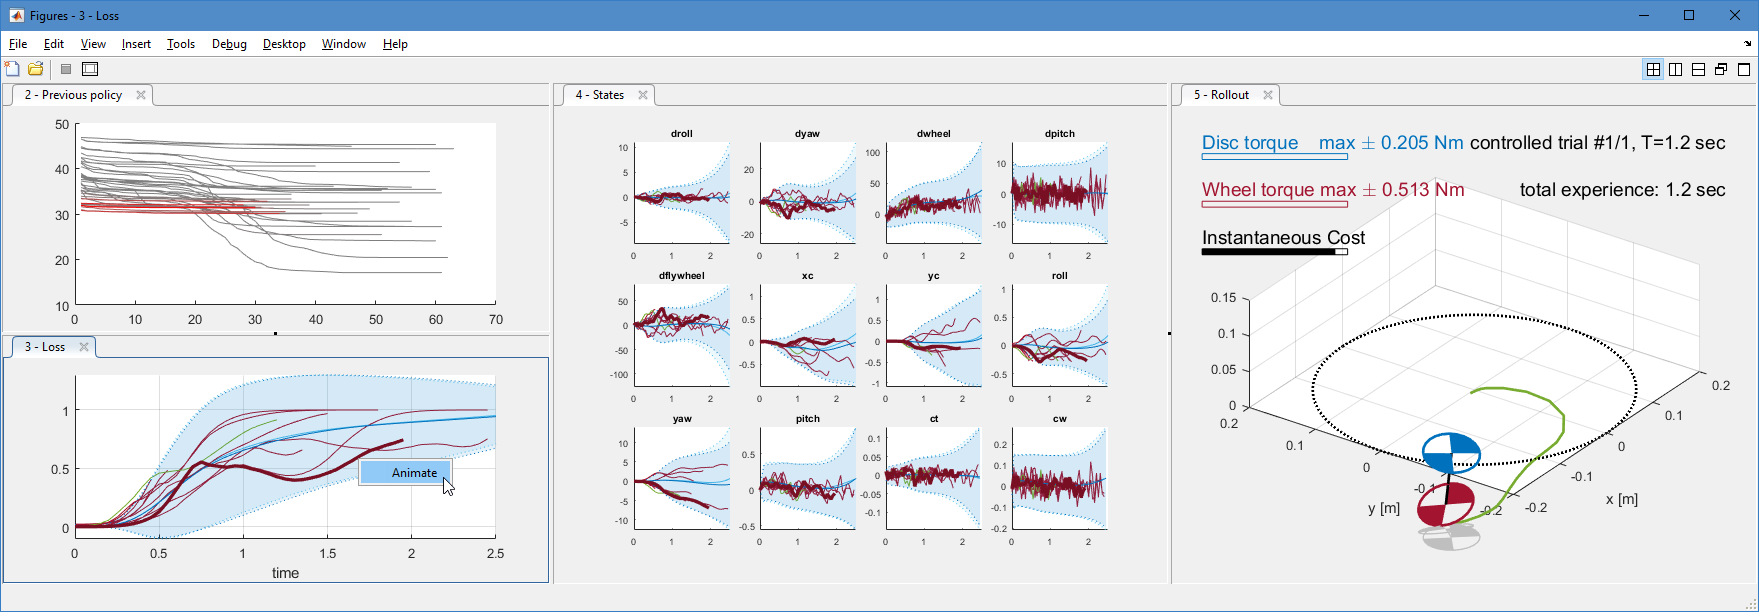
\includegraphics[width=\linewidth]{figures/pilco.png}
		\caption{Screenshot of the \textsc{Pilco} interface}
		\label{fig:pilco-interface}
		\medskip
		\small
		Shown at the end of the project, after the improvements made by the author.
	\end{figure}

	When running this code, the result is a series of state, action, and loss plots, showing simulated and predicted trajectories after each iteration.
	An animation is also played of the trajectory used to train the next iteration of the algorithm.
	Log files are saved containing the state rollouts, controllers, and plots themselves -- making it easy to run the main script on a powerful remote computer, but view the results locally.

	\Cref{fig:pilco-interface} shows an example of the plots.

	\subsection{Embedded C++}

	The embedded code has the following tasks:
	\begin{enumerate}[noitemsep]
		\item Read data from the sensors.
		\item
			Update the internal estimates of orientation from the gyro reading.
			This is done using quaternions as the representation.
		\item Assemble the full state vector from the readings.
		\item Apply the linear control policy.
		\item Store the policy outputs and state data in memory, ready to send back when requested.
	\end{enumerate}
	When being used in conjunction with the Matlab toolbox, the control policy must be updated on each learning iteration, and the output and state data extracted from the robot.
	The process to do this is manual, and consists of the following steps:
	\begin{enumerate}[noitemsep]
		\item Copying the controller parameters into the right place within the C++ code
		\item Recompiling the C++ code
		\item Uploading the binary to the microcontroller
		\item Opening a serial terminal
		\item Manually copying the plaintext output
		\item Saving the copied text into a csv file, which is read by Matlab
	\end{enumerate}
	Of these, steps 2 and 3 are slow, and 1, 5, and 6 are prone to human error.
	Worse still, relying on plaintext in 5 leaves data vulnerable to undetectable corruption through serial line errors\footnotemark. This work therefore comes up with a better approach in \cref{sec:comms}.

	\footnotetext{For instance, if a byte is dropped due to a serial buffer overflow, the number \texttt{10.23} can be read as \texttt{0.23}}

	% TODO

	% From a software design perspective, the code suffered from numerous bad practices:
	% \begin{itemize}
	% 	\item
	% 		\enquote{Magic numbers} -- unnamed numbers in the source code. These ranged from pin numbers, miscellaneous hardware register values, to conversion factors between representations.
	% 		This type of code is impossible to understand without a datasheet for each component in hand.

	% 		The better approach is to use code like \cpp{constexpr double GEARBOX_RATIO = 225/16;} at the top of a file, and use that longer name, rather than repeat \lstinline{225/16} in multiple place.

	% 	\item
	% 		Global variables. This is bad for two reasons: it leaks global state, meaning that attempting to run the program a second time without a full reset is difficult; and it makes it unknowable which variables are used in which locations.

	% 		Generally speaking, variables should be placed in the deepest scope possible. If they must be global, then wrapping related variables up into a \texttt{struct} helps keep things clear
	% \end{itemize}

\end{document}
